\documentclass[xcolor=table, handout]{beamer}

\usepackage{shyne}

% Theme settings
\setbeamertemplate{navigation symbols}{}

\usetheme{Madrid}
\usefonttheme{structurebold}
\usefonttheme[onlymath]{serif}

\AtBeginSection[]
{ 	\begin{frame}{}

	{
	\usebeamerfont{frametitle}
	\begin{beamercolorbox}
		[wd={\textwidth}, center, sep=.2in, rounded=true, shadow=true]
		{frametitle}
	Chapter \thesection\\  \secname 
	\end{beamercolorbox}
	}
	
	\end{frame} 
}

\AtBeginSubsection[]
{ 	\begin{frame}{}

	{
	\usebeamerfont{frametitle}
	\begin{beamercolorbox}
		[wd={\textwidth}, center, sep=.2in, rounded=true, shadow=true]
		{frametitle}
	Section \thesection .\thesubsection\\  \subsecname 
	\end{beamercolorbox}
	}
	
	\end{frame} 
}

\title[Chapter 3]{Stat 201: Statistics I\\ Chapter 3 }
\author[M. Shyne]{}
\institute[Metro State]{
\includegraphics[width=1.75in]{../images/metro_logo}}
\date[8/5/2018]{
\\ \bigskip \bigskip 
\includegraphics[width=.4in]{../images/cc_big}}



\begin{document}
\frame{\titlepage}

% Chapter 3
\setcounter{section}{2}
\section{Statistics for Describing, Exploring, and Combining Data}

% Section 3.1
\subsection{Measures of Center}

\begin{frame}
\frametitle{Measures of center}
\begin{block}{}
\large
In order to understand a data set, values are calculated which summarize the distribution of the data or describe various properties of the data. These are, unsurprisingly, called \bt{descriptive} or \bt{summary} statistics.
\end{block}
\pause
\begin{block}{}
\large
Perhaps the most important of these, \bt{measures of center} are a way of  representing the value of the middle of the data.\\
\medskip
There are four measures of center discussed in this section:
\begin{itemize}
\item mean
\item median
\item mode
\item midrange
\end{itemize} 
\end{block}
\end{frame}

\begin{frame}{Mean}
\begin{block}{}
\large
The \bt{mean} (the arithmetic mean) is the measure of center calculated by adding the values of the data set and dividing by the size of the data set. Also known as the average.
\begin{itemize}
\item Only makes sense with quantitative data
\item Sensitive to outliers (extreme or unusual values) and skewed data distributions.
\end{itemize}
\end{block}

\pause
\begin{block}{To calculate}
Let $X$ be sample of size $n$ of quantitative data with values $\sam x$. Then,
\[\bar x = \frac{\sum x_i}{n}\]
$\bar x$ is the mean of the sample.
\begin{itemize}
\item $\sum$ means add all the $x_i$'s, where $i$ is between 1 and $n$
\end{itemize}
\end{block}
\end{frame}

\begin{frame}{Mean, example}
\begin{exampleblock}{Example}
Suppose we find a sample of 8 students and ask for their ages. 

\begin{itemize}
\item The sample is $X = \set{22, 32, 46, 50, 33, 38, 20, 24}$
\pause\item The sample size is $n=8$
\pause
\item The sum of the data is\\
\smallskip
{\centering
$\sum x_i = 22 + 32 + 46 + 50 + 33 +  38 + 20 + 24 = 265$
\par}
\pause
\item The mean is\\
\smallskip
{\centering
$\ds \bar x = \frac {\sum x_i}{n} = \frac {265} 8 = 33.125 \text{ years}$
\par}
\end{itemize}
\smallskip
\end{exampleblock}
\end{frame}

\begin{frame}{Median}
\begin{block}{}
The \bt{median} is the value that is greater than or equal to at least 50\% of the data and less than or equal to at least 50\% of the data.
\begin{itemize}
\item Can be used with quantitative and ordinal data
\item Not sensitive to extreme values (\bt{resistant} measure of center)
\end{itemize}
\end{block}

\pause
\begin{block}{To calculate}
Arrange the data in order, from lowest to highest.
\begin{itemize}
\item If $n$ is odd, the middle value is the median.
\item If $n$ is even, the median is the mean of the two middle values.
\end{itemize}
\end{block}
\end{frame}

\begin{frame}{Median, example}
\begin{exampleblock}{Example}
Returning to the ages of 8 students.

\begin{itemize}
\item The sample is $X = \set{22, 32, 46, 50, 33, 38, 20, 24}$
\pause
\item Arranged in order, the sample looks like\\
\smallskip
{\centering
$20 \quad 22 \quad 24 \quad 32 \quad 33 \quad 38 \quad 46 \quad 50$
\par}
\pause
\item Since $n$ is even, find the the mean of the two middle values.\\
\smallskip
{\centering
$20 \quad 22 \quad 24  \underbrace{32 \quad 33}_{(32+33)/2 = 32.5}  38 \quad 46 \quad 50$
\par}
\pause
\item The median is $\tilde x = 32.5$ years.
\end{itemize}
\smallskip
\end{exampleblock}

\end{frame}

\begin{frame}{Mean vs. Median}
\begin{exampleblock}{}
\large
Suppose in our age data set, we replaced the $50$ with a $85$.
\begin{itemize}
\item Mean goes from $33.125$ to $37.5$
\item Median remains unchanged at $32.5$
\end{itemize}
\end{exampleblock}

\pause
\begin{block}{}
\large
This is why median is called a \bt{resistant} statistic.
\begin{itemize}
\item Median is used when we don't want a few extreme values to distort a more reasonable middle, such as house prices or incomes.
\end{itemize}
\end{block}
\end{frame}

\begin{frame}{Mean vs. Median, cont.}
\begin{exampleblock}{}
\large
Suppose instead of calculating a grade point average (mean), we calculated a grade point median. Consider a student who got A's in 3 classes and D's in 2.
\begin{itemize}
\item The median grade point is 4, an A.
\item The GPA for such a student would be 2.8.
\end{itemize}
\end{exampleblock}

\pause
\begin{block}{}
\large
The median does not consider all values of a data set. The mean does.
\begin{itemize}
\item Mean is used when all values are important or when we expect to have roughly symmetric data.
\end{itemize}
\end{block}
\end{frame}

\begin{frame}{Mode}
\begin{block}{}
\large
The \bt{mode} is the data value with highest frequency.
\begin{itemize}
\item Can be used with any kind of data.
\item A data set might have more than one mode, or there might not be any mode.
\end{itemize}
\end{block}
\end{frame}

\begin{frame}{Mode, example} 
\begin{exampleblock}{Examples}
\begin{itemize}
\item The age data, $ \set{22, 32, 46, 50, 33, 38, 20, 24}$, has no mode.
\pause
\item From a TACO survey, favorite kind of taco had these responses:\\
\medskip
{\centering
$\set{\text{Beef, Beef, Fish, Shrimp, Beef, Pork, Chicken, Beef, Chicken, Beef}}$
\par}
\medskip
The mode is ``Beef'' with a frequency of five.
\pause
\item Suppose a sample from a class got the following grades on a quiz:\\
\medskip
{\centering
$\set{\text{A, C, B, A, A, B, C, B}}$
\par}
\medskip
The modes are A and B, with frequencies of three each.
\end{itemize}
\end{exampleblock}
\end{frame}

\begin{frame}{Midrange}
\begin{block}{}
\large
The \bt{midrange} is the value half way between the minimum and maximum values. Calculate by finding the mean of the minimum and maximum.
\begin{itemize}
\item Only makes sense with quantitative data.
\item \emph{Very} sensitive the extreme values.
\item Easy to calculate, but rarely used.
\end{itemize}
\end{block}

\pause
\begin{exampleblock}{Example}
The age data is $X = \set{22, 32, 46, 50, 33, 38, 20, 24}$.
\begin{itemize}
\item The minimum age is $20$ and the maximum age is $50$.
\item The midrange is \\
\smallskip
{\centering
$\ds \frac {\min(X) + \max(X)}{2} = \frac {20 + 50}{2} = 35$
\par}
\end{itemize}
\smallskip
\end{exampleblock}

\end{frame}

\begin{frame}{Measures of center in StatCrunch}
\begin{block}{}
\begin{itemize}
\item Stat $\to$ Summary Stats $\to$ Columns
\item Select the column (or columns) which contains the data
\item Under ``Statistics" select statistics to calculate (ctrl-click to select multiple statistics)
\item For measures of center select ``Mean:, ``Median", ``Min", ``Max" and ``Mode"
\item Click ``Compute!"
\item Mean, median and mode will be displayed
\item Midrange must be calculated by hand using min and max
\end{itemize}
\end{block}

\begin{alertblock}{Note}
Mode will display ``No mode", ``Multiple modes" or the mode if exactly one exists. If there are multiple modes, you must identify them yourself.
\end{alertblock}
\end{frame}

\begin{frame}<handout:0>{Group work}
\begin{block}{}
\large
\begin{itemize}
\item For each question, complete part (a).
\end{itemize}
\end{block}
\end{frame}



% Section 3.2
\subsection{Measures of Variation}

\begin{frame}{Other measures}
\begin{block}{}
\large
Other measures are necessary to adequately describe data.
\end{block}
\pause
\bigskip
{\centering
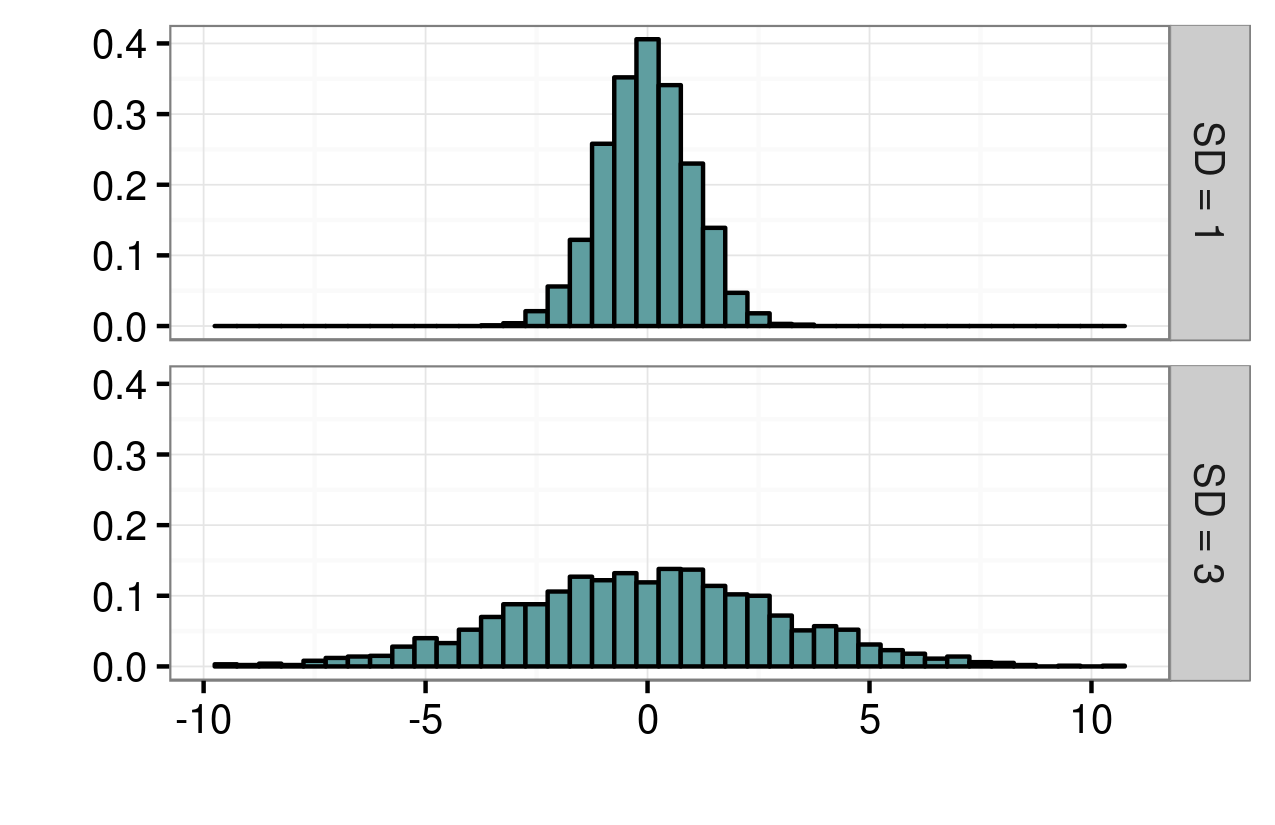
\includegraphics[width=4.25in]{../images/ch03_var_diff}
\par}
\end{frame}

\begin{frame}{Measures of variation}
\begin{block}{}
\large
Another important class of descriptive statistics are \bt{measures of variation} which describe how much the data is spread out.\\
\medskip
There are three measures of variation discussed in this section:
\begin{itemize}
\item Range
\item Variance
\item Standard deviation
\end{itemize}

\end{block}
\end{frame}

\begin{frame}{Range}
\begin{block}{}
\large
The \bt{range} is the difference between the maximum and minimum values.
\begin{itemize}
\item Like the midrange, very sensitive to extreme values.
\end{itemize}
\end{block}

\pause
\begin{exampleblock}{Example}
The age data is $X = \set{22, 32, 46, 50, 33, 38, 20, 24}$.
\begin{itemize}
\item The minimum age is $20$ and the maximum age is $50$.
\pause
\item The range is \\
\smallskip
{\centering
$\max(X) - \min(X) = 50 - 20 = 30 \text{ years}$
\par}
\end{itemize}
\smallskip
\end{exampleblock}

\end{frame}

\begin{frame}{Variance and standard deviation}
\begin{block}{}
\large
The \bt{variance} is the mean of the squared difference of the data from the mean. The \bt{standard deviation} is the square root of the variance.
\begin{itemize}
\pause\item More simply, the standard deviation is the average distance of the data from the data mean (the center).
\pause\item Always non-negative. A zero standard deviation means all the data are the same value.
\pause\item Sensitive to extreme values.
\pause\item The units of standard deviation are the same as the data. Variance units are the data units squared.
\end{itemize}
\end{block}
\end{frame}

\begin{frame}{Variance and standard deviation, calculation}
\begin{block}{To calculate}
Let $X$ be sample of size $n$ of quantitative data with values $\sam x$ and sample mean $\bar x$. Then,\\
\smallskip
{\centering
$\ds \var(X) = s^2 = \frac{\sum (x_i - \bar x)^2}{n-1} \qquad \text{and} \qquad  \f{SD}(X) = s = \sqrt{s^2}$
\par}
\begin{itemize}
\pause\item Note: Never calculate this by hand. Use technology.
\end{itemize}
\end{block}
\end{frame}

\begin{frame}{Variance and standard deviation, example}
\begin{exampleblock}{Example}
The age data is $X = \set{22, 32, 46, 50, 33, 38, 20, 24}$. The sample size is $n=8$ and the sample mean is $\bar x = 33.125$
\begin{itemize}
\pause
\item The variance is 
\begin{align*}
s^2 &= \frac{\sum (x_i - \bar x)^2}{n-1}\\
&= \frac{(22-33.125)^2 + \cdots + (24-33.125)^2}{7}\\
&= 122.125 \text{ years}^\text{2}
\end{align*}
\pause
\item The standard deviation is
\[s = \sqrt{s^2} = \sqrt{122.125} = 11.05 \text{ years}\]
\end{itemize}
\smallskip
\end{exampleblock}
\end{frame}



\begin{frame}{Notation}
\begin{block}{}
\large
Recall, values that describe the properties of populations are called \bt{parameters} and values that describe samples are called \bt{statistics}. Notationally, in math formulas or when abbreviating, Greek letters are used to refer to parameters and Latin letters are used to refer to statistics.
\pause
\begin{center}
\begin{tabular}{c |r l | c}
Property & \multicolumn{2}{c|}{Parameter} & Statistic\\
\hline
Mean & $\mu$ & (mu) & $\bar x$\\
Variance & $\sigma^2$ &(sigma-squared) & $s^2$\\
Standard deviation & $\sigma$ &(sigma) & $s$
\end{tabular}
\end{center} 
\end{block}
\end{frame}

\begin{frame}{Measures of variation in StatCrunch}
\begin{block}{}
\begin{itemize}
\item Stat $\to$ Summary Stats $\to$ Columns
\item Select the column (or columns) which contains the data
\item Under ``Statistics" select statistics to calculate (ctrl-click to select multiple statistics)
\item For measures of variation select ``Variance", ``Std. Dev." and ``Range"
\item Click ``Compute!"
\item The statistics will be displayed
\end{itemize}
\end{block}

\end{frame}

\begin{frame}<handout:0>{Group work}
\begin{block}{}
\large
\begin{itemize}
\item For each question, complete part (b).
\end{itemize}
\end{block}
\end{frame}

% Section 3.3
\subsection{Measures of Relative Standing and Boxplots}

\begin{frame}{Measures of relative standing}
\begin{block}{}
\large
\bt{Measures of relative standing} describe the location of a given data value with a data distribution or a data set.\\
\medskip
Two measures of relative standing are discussed in this section:
\begin{itemize}
\item Z-scores
\item Percentiles
\end{itemize}
\end{block}
\end{frame}

\begin{frame}{Z-scores}
\begin{block}{}
\large
A \bt{z-score} describes the relative position of a data value within a data distribution.
\begin{itemize}
\pause
\item Another way to put it is a z-score is the number of standard deviations that a particular value is above or below the mean.
\pause
\item Z-scores are standardized and unit-less, so they can be used to compare values from different populations.
\pause
\item A positive z-score means the value is greater than the mean and a negative z-score means that it is below the mean. 
\pause
\item Z-scores can be calculated for samples or populations, if the population mean and standard deviation are known.
\end{itemize}
\end{block}
\end{frame}

\begin{frame}{Z-scores, calculations}
\begin{block}{To calculate}
\begin{itemize}
\item For a sample $X$ with sample mean $\bar x$ and standard deviation $s$, the z-score for a value $x$ is
\[z = \frac{x - \bar x}{s}\]
\smallskip
\pause
\item For a population with population mean $\mu$ and standard deviation $\sigma$, the z-score for value $x$ is
\[z = \frac{x - \mu}{\sigma}\]
\end{itemize} 
\end{block}
\end{frame}

\begin{frame}{Z-scores, example}
\begin{exampleblock}{Example}
The age data has mean of $\bar x = 33.125$ and SD of $s=11.05$.
\begin{itemize}
\pause
\item Suppose a new student joins the class. His age is 61. He has an age $z$-score of\\
\smallskip
{\centering
$\ds z = \frac{x - \bar x}{s} = \frac {61-33.125}{11.05} = \frac {27.875}{11.05} = 2.52$
\par}
\medskip
\pause
His age two and a half standard deviations above the class mean.
\smallskip
\pause
\item Another student joins the class. Her age is 27. She has an age $z$-score of\\
\smallskip
{\centering
$\ds z = \frac{x - \bar x}{s} = \frac {27-33.125}{11.05} = \frac {-6.125}{11.05} = -0.554$
\par}
\medskip
\pause
Her age is about a half standard deviation below the class mean.
\end{itemize}

\end{exampleblock}
\end{frame}

\begin{frame}{Values from z-scores}
\begin{block}{}
\large
Sometimes, it is useful to find a value within a data distribution that corresponds to a given z-score. That is, find an $x$ given a $z$. 
\medskip
\begin{itemize}
\pause\item Start with the z-score equation, \\
\smallskip
{\centering $\ds z = \frac{x - \bar x}{s} \txtor z = \frac{x - \mu}{\sigma}$ \par}
\pause\item After some algebra,\\
\smallskip
{\centering $\ds x = \bar x + z s \txtor x = \mu + z \sigma$ \par}
\end{itemize}
\end{block}

\pause
\begin{exampleblock}{Example}
At what age would a student be unusually old? That is, what age corresponds to $z=2$?\\
\medskip
\begin{itemize}
\pause\item $\ds x = \bar x + z s = 33.125 + 2 \times 11.05 =  55.225$ years
\end{itemize}
\end{exampleblock}
\end{frame}

\begin{frame}{Unusual values}

{\centering
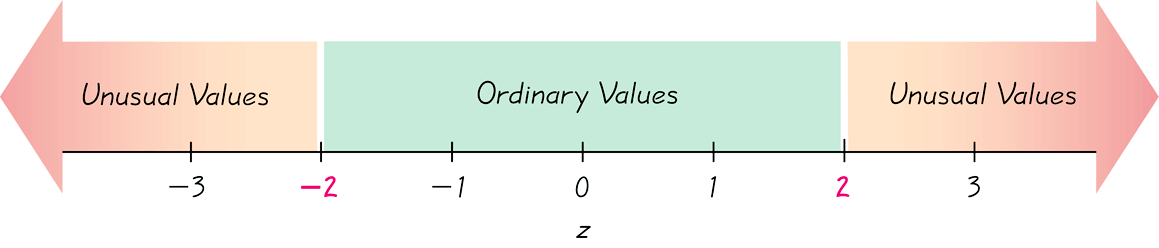
\includegraphics[width=4.5in]{../images/ch03_unusual} \par
}

\begin{block}{}
\large
A value is called \bt{unusual} if it has a z-score $z$ such that $z< -2$ or $z > 2$. A value is \bt{ordinary} if $z$ is between $-2$ and $2$.
\end{block}

\pause
\begin{exampleblock}{Example}
Consider the new students to the class:
\begin{itemize}
\item The 61 year old ($z=2.52$) has an unusual age for the class. 
\item The 27 year old ($z=-0.554$) has an ordinary age for the class.
\end{itemize}
\end{exampleblock}
\end{frame}

\begin{frame}{Percentiles}
\begin{block}{}
\large
\bt{Percentiles} measure relative position within a data set as order rank. In other words, the value at the $p$th percentile (written as $P_p$) in a data set is greater than $p$\% of the data.
\end{block}

\pause
\begin{block}{To calculate}
\begin{itemize}
\item To find the percentile of a value $x$ in a data set,\\
\smallskip
{\centering
$\ds \%\text{ile} = \frac{\text{number of values} < x}{n} \times 100\%$
\par}
\medskip
If percentile is not a whole number, round up.
\medskip
\pause\item To find the value of $P_p$ (the $p$th percentile), calculate the rank,\\
\smallskip
{\centering
$\ds r = \frac p {100} \times n$
\par}
\medskip
If $r$ is a whole number, $P_p$ is the mean of the $r$th and $(r+1)$th values. If not, round up. Then, $P_p$ is the $r$th value in an ordered list.
\end{itemize}
\end{block}
\end{frame}

\begin{frame}{Percentile, example}
\begin{exampleblock}{Example}
The age data, in order is, \\
\smallskip
{\centering
$20 \quad 22 \quad 24 \quad 32 \quad 33 \quad 38 \quad 46 \quad 50$
\par}

\begin{itemize}
\pause
\item The percentile of the value 38 is\\
\medskip
{\centering
$\ds \frac{\text{number of values} < x}{n} \times 100\% = \frac{5}{8} \times 100\% = 62.5 \,\% \implies P_{63}$
\par} 
\medskip
\pause\item To find the 30th percentile, $P_{30}$, calculate rank\\
\medskip
{\centering
$\ds r= \frac {p}{100} \times n = \frac {30}{100} \times 8 = 2.4 $
\par}
\medskip
Round up $r$ to $3$. $P_{30}$ is the 3rd value, $24$.
\end{itemize}
\end{exampleblock}
\end{frame}

\begin{frame}{Percentiles in StatCrunch}
\begin{block}{}
To find percentile of value $x$:
\begin{itemize}
\item If data is not ordered, order it using Data $\to$ Sort
\item The row number of the value \bt{before} $x$ is number of values $< x$
\item The row number of the last value is $n$
\item Use the formula to calculate percentile (round up)
\end{itemize}
To find value for percentile $p$:
\begin{itemize}
\item Stat $\to$ Summary Stats $\to$ Columns
\item Select the column (or columns) which contains the data
\item Under ``Percentiles..." enter $p$ (can enter multiple $p$'s separated by commas)
\item Click ``Compute!"
\item The value(s) will be displayed as ``$p$th Per."
\end{itemize}
\end{block}
\end{frame}


\begin{frame}{Quartiles}
\begin{block}{}
\large
The \bt{quartiles} are values that divide the data set into 4 parts, or quarters.\\
\smallskip
{\centering
$Q_1 = P_{25} \qquad Q_2 = P_{50} \qquad Q_3 = P_{75}$
\par}
\begin{itemize}
\pause
\item Note: The median is equivalent to $Q_2$ and $P_{50}$.
\end{itemize}
\end{block}
\end{frame}

\begin{frame}{5 number summary}
\begin{block}{}
\large 
The \bt{5 number summary} summarize the distribution of a data set.\\
\medskip
The 5 numbers are:
\begin{itemize}
\item Minimum
\item $Q_1$
\item Median (or $Q_2$)
\item $Q_3$
\item Maximum
\end{itemize}
\end{block}
\end{frame}

\begin{frame}{5 number summary, example}
\begin{exampleblock}{Example}
The age data, in order is, 
\[20 \quad 22 \quad 24 \quad 32 \quad 33 \quad 38 \quad 46 \quad 50 \]
The 5 number summary is
\[\underbrace{20}_{\min} \quad \underbrace{23}_{Q_1} \quad \underbrace{32.5}_{\f{med}} \quad \underbrace{42}_{Q_3} \quad \underbrace{50}_{\max}\]
\end{exampleblock}
\end{frame}

\begin{frame}{Boxplots}
\begin{block}{}
\large
A \bt{boxplot} is a graph depicting the 5 number summary.
\end{block}
{\centering
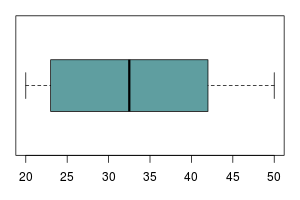
\includegraphics[width=4in]{../images/ch03_boxplot}\par
}
\end{frame}

\begin{frame}{Five number summaries in StatCrunch}
\begin{block}{}
\begin{itemize}
\item Stat $\to$ Summary Stats $\to$ Columns
\item Select the column (or columns) which contains the data
\item Under ``Statistics" select ``Min", ``Q1", ``Median", ``Q3" and ``Max"
\item Or, under ``Percentile" enter ``1, 25, 50, 75, 99" (might not give correct values for the min and max in large data sets)
\item Click ``Compute!"
\item The values will be displayed, but maybe not in the right order
\end{itemize}
\end{block}

\end{frame}

\begin{frame}{Boxplots in StatCrunch}
\begin{block}{}
\begin{itemize}
\item Graph $\to$ Boxplot
\item Select the column (or columns) which contains the data
\item (Optional) Under ``Other options", click ``Draw boxes horizontally"
\item Click ``Compute!"
\item Hold pointer over plot to get IQR (inter-quartile range) and five number summary
\end{itemize}
\end{block}

\end{frame}

\begin{frame}<handout:0>{Group work}
\begin{block}{}
\large
\begin{itemize}
\item For each question, complete part (c).
\end{itemize}
\end{block}
\end{frame}


\end{document}